% ОБЯЗАТЕЛЬНО ИМЕННО ТАКОЙ documentclass!
% (Основной кегль = 14pt, поэтому необходим extsizes)
% Формат, разумеется, А4
% article потому что стандарт не подразумевает разделов
% Глава = section, Параграф = subsection
% (понятия "глава" и "параграф" из стандарта)
\documentclass[a4paper,article,14pt]{extarticle}

% Подключаем главный пакет со всем необходимым
\usepackage{spbudiploma}

\usepackage{graphicx}
\usepackage{float}
\usepackage{textcomp}
\usepackage{subcaption}

\usepackage{tikz}
\usetikzlibrary{positioning}
 
\begin{document} % начало документа

% Титульник в файле titlepage_ru.tex
% --------------------- Стандарт СПбГУ для ВКР --------------------------
% Автор: Тоскин Николай, itonik@me.com
% Если заметили ошибку, напишите на email
% Если хотите добавить изменение самостоятельно, GitHub: . PR-s welcome!
% Использованы материалы:
% habr.com/ru/post/144648/
% cpsconf.ru
% Текст:
% http://edu.spbu.ru/images/data/normativ_acts/local/20181030_10432_1.pdf
% Титульный лист:
% http://edu.spbu.ru/images/data/normativ_acts/local/20180703_6616_1.pdf
% -----------------------------------------------------------------------

% Титульный лист диплома СПбГУ
% Временное удаление foot на titlepage
\newgeometry{left=30mm, top=20mm, right=15mm, bottom=20mm, nohead, nofoot}
\begin{titlepage}
\begin{center}
% Первый символ съедается, первым знаком поставлен Ы
\textbf{Санкт--Петербургский}
\textbf{государственный университет}

\vspace{35mm}

\textbf{\textit{\large ПОТТЕР Гарри Джеймсович}} \\[8mm]
% Название
\textbf{\large Выпускная квалификационная работа}\\[3mm]
\textbf{\textit{\large Оптимизация заклятий в распределенной сети
мозгошмыг}}

\vspace{20mm}
% Булшит
Уровень образования: бакалавриат\\
Направление 01.03.02 «Прикладная математика и информатика»\\
Основная образовательная программа СВ.5005.2015
«Прикладная математика, фундаментальная информатика и программирование»\\
Профиль «Исследование и проектирование систем управления\\ и обработки сигналов»\\[30mm]


% Научный руководитель, рецензент
% Сходить в уч отдел и узнать, правильно ли
\begin{flushright}
{Научный руководитель:} \\
профессор, кафедра компьютерных технологий \\ и систем, д.ф. - м.н.  Веремей~Евгений Игоревич
\end{flushright}
\begin{flushright}
{Рецензент:} \\
профессор, кафедра компьютерных технологий \\и систем, д.ф. - м.н.  Веремей~Евгений Игоревич
\end{flushright}

\vfill 

{Санкт-Петербург}
\par{2019 г.}
\end{center}
\end{titlepage}
% Возвращаем настройки geometry обратно (то, что объявлено в преамбуле)
\restoregeometry
% Добавляем 1 к счетчику страниц ПОСЛЕ titlepage, чтобы исключить 
% влияние titlepage environment
\addtocounter{page}{1}

% Титульник в файле titlepage_en.tex
% --------------------- Стандарт СПбГУ для ВКР --------------------------
% Автор: Миронов Алексей
% Использованы материалы:
% habr.com/ru/post/144648/
% cpsconf.ru
% Текст:
% http://edu.spbu.ru/images/data/normativ_acts/local/20181030_10432_1.pdf
% Титульный лист:
% http://edu.spbu.ru/images/data/normativ_acts/local/20180703_6616_1.pdf
% -----------------------------------------------------------------------

% Титульный лист диплома СПбГУ
% Временное удаление foot на titlepage
\newgeometry{left=30mm, top=20mm, right=15mm, bottom=20mm, nohead, nofoot}
\begin{titlepage}
\begin{center}
% Первый символ съедается, первым знаком поставлен Ы
\normalsize{Saint Petersburg State University}\\
\normalsize{Applied Mathematics and Computer Science}\\
\normalsize{The chair of applied cybernetics}

\vspace{35mm}

\normalsize{Mironov Alexey Vladislavovich} \\[8mm]
% Название
\large{Analytical estimates of the pull-in range for third-order PLLs}\\[3mm]
\small{Final qualifying work}

\vspace{50mm}

% Научный руководитель, рецензент
% Сходить в уч отдел и узнать, правильно ли
\begin{flushright}
{Scientific supervisor:} \\
assistant professor Yuldashev~R.\:V.
\end{flushright}
\begin{flushright}
{Reviewer:} \\
Blagov~M.\:V.
\end{flushright}

\vfill 

{Saint--Petersburg}
\par{\number\year}
\end{center}
\end{titlepage}
% Возвращаем настройки geometry обратно (то, что объявлено в преамбуле)
\restoregeometry
% Добавляем 1 к счетчику страниц ПОСЛЕ titlepage, чтобы исключить 
% влияние titlepage environment
\addtocounter{page}{1}
 
\tableofcontents


%%%%%%%%%%%%%%%%%%%%%%%%%%%%%%%%%%%%%%%%%%%%%%%%%%%%%%%%%%%%%%%%%%%%%%%
%%%%%%%                         ВВЕДЕНИЕ                        %%%%%%%
%%%%%%%%%%%%%%%%%%%%%%%%%%%%%%%%%%%%%%%%%%%%%%%%%%%%%%%%%%%%%%%%%%%%%%%

\pagebreak
\section{Введение}
В различных системых, например телекоммуникационных, часто возникает необходимость в синхронизации частот. В гражданских системах связи, таких как радио или телевидение, используется одна несущая частота, которая является постоянной. Многие люди даже знают частоту вещания своей любимой радиостанции. Однако для военных нужд использование одной несущей частоты несет определенные риски, связанные с тем, что постоянную частоту легко заглушить. Для решения этой проблемы военными был разработан метод скачкообразного изменения частоты сигнала \cite{ghulam}. Для этого выбирается $N$ различных частот, которые чередуются с некоторым интервалом. Для приемника сигнала это означает, что он должен уметь подстраиваться под несущую частоту очень быстро, т.е. возникает необходимость в синхронизации частоты трансмиттера и ресивера. 

Синхронизация частот требуется не только в телекоммуникационных системах, но и в компьютерах. С развитием микропроцессоров, когда тактовая частота достигла 50МГц, появилась необходимость устранять задержку между внешними и внутренними тактами (Clock skew), вызванную задержкой драйвера встроенного тактового генератора. Поскольку размер микропроцессора увеличился до 1 миллиона транзисторов, и кроме того, возросла нагрузка на генератор тактов. Все это привело к тому, что задержка тактового генератора может составлять более 2 наносекунд \cite{Microprocessors}. Эта задержка вызывает большое время удержания для входных/выходных сигналов и является ограничением проектирования систем на высоких тактовых частотах. Возникает необходимость в синхронизации частоты внутренних и внешних тактов. 

Для решения проблемы расфазировки в первой половине XX века была изобретена система фазовой автоподстройки частоты \cite{appleton} (ФАПЧ)~--- система с обратной связью, используемая для синхронизации частот сигналов эталонного и подстраиваемого генератора, в простейшем виде состоящая из фазового детектора (компаратора), фильтра нижних частот и генератора, управляемого напряжением. Сразу после появления системы ФАПЧ начали применяться в радио и телевидении \cite{blagov}. Инженерная практика применения и теория систем ФАПЧ начали интенсивно развиваться во второй половине XX века \cite{seledji}. Сразу после реализации систем фазовой автоподстройки частоты в виде одной микросхемы системы ФАПЧ стали широко применяться в современных телекоммуникационных системах. В настоящее время микросхемы, использующие системы фазовой автоподстройки, используются в различных электромеханических приборах \cite{best}, энергетических генераторах, системах передачи данных \cite{ashari} и навигационных системах \cite{rao} (GPS, ГЛОНАСС и Галилео).

Особенностью функционирования систем ФАПЧ является нелинейность фазы подстраиваемого генератора в переходном режиме \cite{kuznetsov_nonlinear}. При постоянной частоте эталонного генератора система ФАПЧ позволяет получить различные степени синхронизации. Например, система ФАПЧ второго порядка теоретически позволяет получить полную синхронизацию сигналов, т.е. сигнал с той же частотой и постоянную разность фаз. Одним из недостатков систем ФАПЧ второго порядка является недостаточное подавление высокочастотного шума, который может существенно повлиять на функционирование системы в целом. Еще одним недостатком является резкое ухудшение синхронизации частот при изменении коэффициента передачи. Именно поэтому наряду с системами ФАПЧ второго порядка исследуются системы третьего порядка. Основными преимуществами ФАПЧ третьего порядка является хорошее подавление шума и более низкая стационарная ошибка по сравнению с системами ФАПЧ второго порядка \cite{thirdOrderPLL}. В различных телекоммуникационных системах точность синхронизации является одним из важнейших параметров, поскольку именно от точности подстройки зависит производительность системы \cite{UsageOfThirdOrder1}. Однако с увеличением точности синхронизации возрастает сложность реализации и анализа систем фазовой автоподстройки частоты. 

Основными параметрами ФАПЧ являются полосы удержания, захвата и захвата без проскальзывания \cite{shahgildyan}. В данной работе получены оценки полосы захвата для некоторых систем фазовой автоподстройки частоты третьего порядка. Такие системы исследовались в \cite{kuznetsov_article}, для них были получены численные оценки полосы захвата. Так же оценки полосы захвата для систем ФАПЧ третьего порядка были представлены в \cite{kuznetsov}. Однако в данной работе получены аналитические оценки полосы захвата, которые были подтверждены численно. Так же восстановлен вывод для оценки, полученной в \cite{kuznetsov}.

%%%%%%%%%%%%%%%%%%%%%%%%%%%%%%%%%%%%%%%%%%%%%%%%%%%%%%%%%%%%%%%%%%%%%%%
%%%%%%%              Математическая модель ФАПЧ                 %%%%%%%
%%%%%%%%%%%%%%%%%%%%%%%%%%%%%%%%%%%%%%%%%%%%%%%%%%%%%%%%%%%%%%%%%%%%%%%

\newpage
\section{Математическая модель ФАПЧ и основные понятия}
Рассмотрим синхронизацию колебаний на примере классической системы фазовой автоподстройки частоты Рис. \ref{PLL-img}.
\begin{figure}[H]
\begin{center}
\resizebox{\textwidth}{!}{%
\begin{tikzpicture}
\node at (0.5,0) [draw, text width=3cm, align=center, rectangle] (a) {Фазовый детектор \\ (компаратор)};
\node at (5.2,0) [draw, label=below:{Фильтр}, align=center, rectangle] (loop_filter) {$W(s)$};
\node at (10.5,0) [draw, label={[align=center]below:Генератор,\\управляемый напряжением}] (VCO) {$\omega_{vco}(t) = \omega_{vco}^{free}+K_{vco}\upsilon_f(t)$};

\draw[->] (-3.3,0) -- (a.west) node[midway,above,inner sep=2pt] {sin($\omega_{ref}t$)};
\draw[->] (a.east) -- (loop_filter.west) node[midway,above,inner sep=1pt] {$\upsilon_e(\omega_{e}t)$};
\draw[->] (loop_filter.east) -- (VCO.west) node[midway,above,inner sep=2pt] {$\upsilon_f(t)$};
\draw[->] (VCO.east) -- (17,0) node[midway,above,inner sep=2pt] {cos($\omega_{vco}t$)};
\draw[->] (15,0) --  +(0,-2) --  +(-14.5,-2) --  (a.south);

\end{tikzpicture}
}
\end{center}
\caption{Схема классической системы ФАПЧ, где $\omega_{ref}$~--- частота опорного сигнала, $\omega_{vco}$~--- частота сигнала ГУН, $\upsilon_f(t)$~--- выходной сигнал фильтра, $\omega_{vco}^{free}$~--- частота свободных колебаний ГУН, $\upsilon_e(\omega_{e}t)$~-- характеристика фазового детектора, $\omega_e = \omega_{ref}-\omega_{vco}$ \label{PLL-img}}
\end{figure}

Опорный сигнал подается на вход кольца ФАПЧ. Фазовый детектор (компаратор) принимает опорный сигнал и сигнал генератора, управляемого напряжением, в результате воздействия на выходе компаратора имеем:
 \begin{equation*}
 \begin{aligned}
\upsilon_e(\theta_{ref}(t) - \theta_{vco}(t)),
 \end{aligned}
\end{equation*}
где $\theta_{vco}(t)$~--- фаза подстраиваемого генератора, $\theta_{ref}(t)$~--- фаза эталонного генератора, $\upsilon_e(\theta_e(t))$~--- характеристика фазового детектора, являющаяся $2\pi$-периодической функцией. Функцию
 \begin{equation}\label{phase_error}
 \begin{aligned}
\theta_e(t) = \theta_{ref}(t) - \theta_{vco}(t)
 \end{aligned}
\end{equation}
называют фазовой ошибкой.

Сигнал, полученный на выходе компаратора $\upsilon_e(\theta_e(t))$, поступает на вход фильтра нижних частот. Связь входного $\upsilon_e(\theta_e(t))$ и выходного $\upsilon_f(t)$ сигналов фильтра нижних частот может быть описана уравнениями:
 \begin{equation}\label{linear_block_eq}
 \begin{aligned}
&\dot{x} = Ax + B\upsilon_e(\theta_e(t))\\
&\upsilon_f(t) = C^Tx + D\upsilon_e(\theta_e(t)),
 \end{aligned}
\end{equation}
где $A$~--- постоянная матрица $n \times n$, $B, C \in \mathbb{R}^n$  постоянные $n$-мерные векторы, $D$~--- константа, $x(t) \in \mathbb{R}^n$~--- вектор состояний системы. Для практических применений инженерами были физически реализованы аналоговые фильтры в виде RL-цепей, RLC-цепей и др.

Выходной сигнал фильтра нижних частот поступает на вход генератора, управляемого напряжением:
 \begin{equation}\label{VCO_eq}
 \begin{aligned}
\dot{\theta}_{vco}(t) = \omega_{vco}(t) = \omega^{free}_{vco} + K_{vco}\upsilon_f(t),
 \end{aligned}
\end{equation}
где $\omega^{free}_{vco}$~--- частота свободных колебаний ГУН, $K_{vco}$~--- коэффициент передачи. При этом полагаем, что эталонный генератор работает на постоянной частоте:
 \begin{equation}
 \begin{aligned}
\dot{\theta}_{ref}(t) = \omega_{ref}(t) \equiv \omega_{ref}.
 \end{aligned}
\end{equation}
Разность между частотой эталонного генератора и частотой свободных колебаний ГУН обозначим:
 \begin{equation}\label{constant_frequency}
 \begin{aligned}
\omega_e^{free} \equiv \omega_{ref} - \omega^{free}_{vco}.
 \end{aligned}
\end{equation}
Из \eqref{phase_error} и \eqref{linear_block_eq}-\eqref{constant_frequency} получим систему дифференциальных уравнений, описывающих ФАПЧ:
 \begin{equation}\label{pllequations}
 \begin{aligned}
 &\dot{x} = Ax + B\upsilon_e(\theta_e)\\
 &\dot{\theta}_e = \omega_e^{free} - K_{vco}(C^Tx + D\upsilon_e(\theta_e)).
 \end{aligned}
\end{equation}
В системе \eqref{pllequations} сделаем преобразования $-K_{vco}C \rightarrow C$, $-K_{vco}D \rightarrow D$. Тогда система \eqref{pllequations} принимает вид:
 \begin{equation}\label{pllequations-1}
 \begin{aligned}
 &\dot{x} = Ax + B\upsilon_e(\theta_e)\\
 &\dot{\theta}_e = \omega_e^{free} - C^Tx + D\upsilon_e(\theta_e).
 \end{aligned}
\end{equation}
В системе \eqref{pllequations-1} сделаем замену:
 \begin{equation}
 \begin{aligned}
 &z = x + A^{-1}B\gamma \\
 &\gamma = \frac{\omega_e^{free}}{C^TA^{-1}B-D}.
 \end{aligned}
\end{equation}
В результате преобразований получим систему:
 \begin{equation}\label{system_pll}
 \begin{aligned}
 &\dot{z} = Az + B(\upsilon_e(\theta_e) - \gamma)\\
 &\dot{\theta_e} = C^Tz + D(\upsilon_e(\theta_e) - \gamma)).
 \end{aligned}
\end{equation}

В данной работе будем рассматривать систему ФАПЧ с характеристикой фазового детектора $\upsilon_e(\theta_e) = \operatorname{sin}(\theta_e)$. Системы ФАПЧ с характеристикой фазового детектора $\operatorname{sin}(\theta_e)$ применяются в GPS ресиверах \cite{kaplan}. Тогда система \eqref{system_pll} принимает вид:
 \begin{equation}\label{system}
 \begin{aligned}
 &\dot{z} = Az + B(\operatorname{sin}(\theta_e) - \gamma)\\
 &\dot{\theta_e} = C^Tz + D(\operatorname{sin}(\theta_e) - \gamma)).
 \end{aligned}
\end{equation}
Введем определение полосы захвата согласно \cite{kuznetsov_article}.
\begin{definition}
Система \eqref{system} называется глобально асимптотически устойчивой, если любое решение $x(t, x_0)$  стремится к некоторому состоянию равновесия при $t \rightarrow +\infty$.
\end{definition}

\begin{definition}
Полоса захвата~--- максимальная разность по модулю частот опорного сигнала и ГУН $|\omega_p|$ такая, что система \eqref{system} глобально асимптотически устойчива для всех $\omega_e^{free} \in [0, |\omega_p|)$.
\end{definition}

\begin{definition}
Комплекснозначная функция  
\begin{equation}
 \begin{aligned}
 W(s)=C^T \left(A-sI\right)^{-1}B - D
 \end{aligned}
\end{equation}
называется передаточной функцией фильтра.
\end{definition}

Рассмотрим систему \eqref{system_pll}. Положим что функция $\upsilon_e(\theta_e)$ непрерывно  дифференцируема на $\mathbb{R}$ и удовлетворяет условиям:
\begin{equation}
 \begin{aligned}
 \mu_1 \leqslant \frac{d \upsilon_e(\theta_e)}{d \theta_e} \leqslant \mu_2, \quad \forall \theta_e \in \mathbb{R}.
 \end{aligned}
\end{equation}
Введем в рассмотрение число:
 \begin{equation}\label{nu}
 \begin{aligned}
\nu = \int_{0}^{2\pi}\left( \upsilon_e(\theta_e) - \gamma \right)d\theta_e \left( \int_{0}^{2\pi} \mid \upsilon_e(\theta_e) - \gamma \mid d\theta_e \right)^{-1}.
 \end{aligned}
\end{equation}
Следующая теорема дает условие глобальной асимптотической устойчивости \eqref{system}.
\begin{theorem}[\cite{leonov}]\label{th1}
Пусть все нули функции $\upsilon_e(\theta_e) - \gamma$ изолированы, пара $(A, B)$ вполне управляема, все собственные значения матрицы $A$ имеют отрицательные вещественные части и существуют числа $\varepsilon > 0, \delta > 0, \tau \geqslant 0$, и $\varkappa$, такие что имеют место неравенства:
 \begin{align}
 &\operatorname{Re}\left( \varkappa W(ix)- \varepsilon\left[W(ix)\right]^2-\tau\left[ 	
\overline{W(ix)}-\mu_1^{-1} ix \right]\left[W(ix)+\mu_2^{-1} ix \right]\right) \geqslant \delta, \notag \\
&\hspace{385pt minus 1fil} \forall x \in \mathbb{R} \label{first_th_eq0} \\
&\varepsilon\delta > (\varkappa\nu)^2. \label{second_th_eq0}
 \end{align}
 Тогда система \eqref{system} глобально асимптотически устойчива.
\end{theorem}

При $\upsilon_e(\theta_e) = \operatorname{sin}(\theta_e)$, очевидно что $\mu_1 = -1$, $\mu_2 = 1$. Условия теоремы \eqref{first_th_eq0} и \eqref{second_th_eq0} принимают следующий вид соответственно:
 \begin{align}
&\operatorname{Re}\left( \varkappa W(ix)- \varepsilon\left[W(ix)\right]^2-\tau\left[ \overline{W(ix)}+ix \right]\left[W(ix)+ix \right]\right) \geqslant \delta \text{,} \quad
\forall x \in \mathbb{R} \label{first_th_eq}\\
&\varepsilon\delta > (\varkappa\nu)^2.\label{second_th_eq}
 \end{align}
Подставим $\upsilon_e(\theta_e) = \operatorname{sin}(\theta_e)$ в \eqref{nu}, тогда $\nu$ определяется следующим образом:
 \begin{equation}
 \begin{aligned}
\mid\nu\mid = \frac{0,5\pi\gamma}{\gamma \operatorname{arcsin} (\gamma) + \sqrt{1-\gamma^2}}.
 \end{aligned}
\end{equation}

%%%%%%%%%%%%%%%%%%%%%%%%%%%%%%%%%%%%%%%%%%%%%%%%%%%%%%%%%%%%%%%%%%%%%%%
%%%%%%%                   Постановка задачи                     %%%%%%%
%%%%%%%%%%%%%%%%%%%%%%%%%%%%%%%%%%%%%%%%%%%%%%%%%%%%%%%%%%%%%%%%%%%%%%%

\newpage
\section{Постановка задачи}
Для физической реализации систем фазовой автоподстройки частоты инженерам необходимо проводить анализ их устойчивости. Исследования локальной устойчивости ФАПЧ обычно проводится с использованием хорошо известных инженерам критериев: Эрмита-Михайлова, Рауса-Гурвица, Харитонова и др. Однако для инженеров также важно определять полосу захвата, которая определяется областью параметров, обеспечивающей глобальную устойчивость системы. Опираясь на частотный критерий глобальной устойчивости, предложенный Г. А. Леоновым, получим оценки полосы захвата для систем фазовой автоподстройки частоты со следующими передаточными функциями фильтра: 
 \begin{align}
&W(s) = \frac{1}{(1+\tau_{p1}s)(1+\tau_{p2}s)},\\[5pt]
&W(s) = \frac{(1+\tau_{z1}s)^2}{(1+\tau_{p1}s)^2},\\[5pt]
&W(s) = \frac{(1+\tau_{z1}x)(1+\tau_{z2}x)}{(1+\tau_{p1}x)(1+\tau_{p2}x)},\\
&0<\tau_{pi},\tau_{zj} < 1, \quad \tau_{pi} \neq \tau_{zj}, \quad i=1,2, \quad j=1,2.
 \end{align}
 
 Для оценки полосы захвата будем выбирать $\varepsilon, \delta, \varkappa, \tau$, удовлетворяющие \eqref{first_th_eq} и \eqref{second_th_eq} так, чтобы максимизировать $\nu$. Из максимальности $\nu$ получим максимальный $\omega_e^{free}$, при котором система \eqref{system} глобально асимптотически устойчива.
 
%%%%%%%%%%%%%%%%%%%%%%%%%%%%%%%%%%%%%%%%%%%%%%%%%%%%%%%%%%%%%%%%%%%%%%%
%%%%%%%                      ФИЛЬТР 1                           %%%%%%%
%%%%%%%%%%%%%%%%%%%%%%%%%%%%%%%%%%%%%%%%%%%%%%%%%%%%%%%%%%%%%%%%%%%%%%%

\pagebreak
\section{Основные результаты}

\subsection{Оценка полосы захвата для систем ФАПЧ с фильтром $\frac{1}{(1+\tau_{p1}s)(1+\tau_{p2}s)}$}
Оценим полосу захвата для систем ФАПЧ с фильтром, определяемым передаточной функцией:
 \begin{equation}\label{filter1}
 \begin{aligned}
W(s) = \frac{1}{(1+\tau_{p1}s)(1+\tau_{p2}s)} = \frac{1}{1+as + bs^2}, \quad 0<\tau_{p1},\tau_{p2} < 1,
 \end{aligned}
\end{equation}
где $a = \tau_{p1}+\tau_{p2}$, $b = \tau_{p1}\tau_{p2}$. Рассмотрим первое условие теоремы \ref{th1}. Подставим \eqref{filter1} в \eqref{first_th_eq} и перенесем все в левую часть неравенства. Сделаем замену переменной $t = s^2$. Не умаляя общности, можем положить $\varkappa = 1$. В результате преобразований \eqref{first_th_eq} принимает вид:
\begin{equation}\label{first_condition}
 \begin{aligned}
&\tau b^2t^3 + (\tau a^2-2 \tau b - \delta b^2)t^2 + (- b+\tau-\delta a^2 + 2\delta b)t +\\
&+ (1-\varepsilon-\tau-\delta) \geqslant 0, \quad \forall t \in \mathbb{R_+}.
 \end{aligned}
\end{equation}
Неравенство $1 - \varepsilon - \tau - \delta \geqslant 0$ является необходимым условием справедливости \eqref{first_condition}. Для максимизации $\nu$ положим $\varepsilon = 1 - \tau - \delta$. Тогда \eqref{first_condition} принимает вид:
\begin{equation}\label{ineq1} 
 \begin{aligned}
&\tau b^2t^2 + (\tau a^2-2 \tau b - \delta b^2)t + (- b+\tau-\delta a^2 + 2\delta b) \geqslant 0 \text{,}\quad \forall t \in \mathbb{R_+}.
 \end{aligned}
\end{equation}
Введем обозначения:
\begin{equation}
 \begin{aligned}
\widetilde A = \tau b^2, \quad 
\widetilde B = \tau a^2-2 \tau b - \delta b^2, \quad
\widetilde C = - b+\tau-\delta a^2 + 2\delta b.
 \end{aligned}
\end{equation}
Заметим, что для выполнения \eqref{ineq1} необходимо потребовать $\widetilde A \geqslant 0$ и $\widetilde C \geqslant 0$, откуда следует $\widetilde B \geqslant 0$. Подставим $\varepsilon = 1 - \tau - \delta$, $\varkappa = 1$ в \eqref{second_th_eq} и выразим $\nu^2$, тогда \eqref{second_th_eq} принимает вид:
\begin{equation}\label{extr_filter1}
 \begin{aligned}
\nu^2 < 4\delta-4\tau\delta - 4\delta^2.
 \end{aligned}
\end{equation}
Максимизируем \eqref{extr_filter1} при условии $\widetilde C \geqslant 0$.  Заметим, что максимальное значение достигается на границе или в точках понижения ранга. Вычислим градиент \eqref{extr_filter1}:
\begin{equation}
 \begin{aligned}
(4 - 4\tau - 8\delta, 4\delta).
 \end{aligned}
\end{equation} 
Точка понижения ранга: $\delta = 0, \tau = 1$. Это противоречит условию теоремы $\delta > 0$. Рассмотрим границу допустимой области $\widetilde C = 0$, выразим $\tau$ и подставим в \eqref{extr_filter1}:
\begin{equation}\label{one_var_max}
 \begin{aligned}
\nu^2 < 4\delta(1 - b) - 4\delta^2(a^2 -2b +1)\\
 \end{aligned}
\end{equation} 
Максимум  \eqref{one_var_max} достигается при $\delta = \frac{1-b}{2(a^2 - 2b + 1)}$ и равен:
\begin{equation}\label{filter1_max}
 \begin{aligned}
\nu^2 < \frac{(b - 1)^2}{a^2 - 2b + 1} = \frac{(\tau_{p1}\tau_{p2} - 1)^2}{\tau_{p1}^2 + \tau_{p2}^2 + 1}.
 \end{aligned}
\end{equation} 

\begin{figure}[H]
\begin{subfigure}{.5\textwidth}
  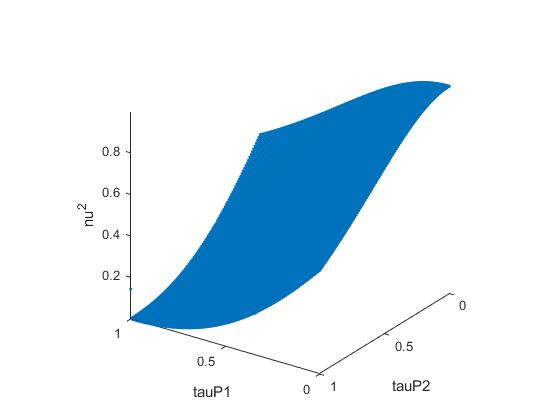
\includegraphics[width=9cm]{images/filter1_exact.jpg}
  \caption{Численная оценка $\nu^2$ в MATLAB с помощью функции fmincon.}
  \label{fig:sub1}
\end{subfigure}%
\begin{subfigure}{.5\textwidth}
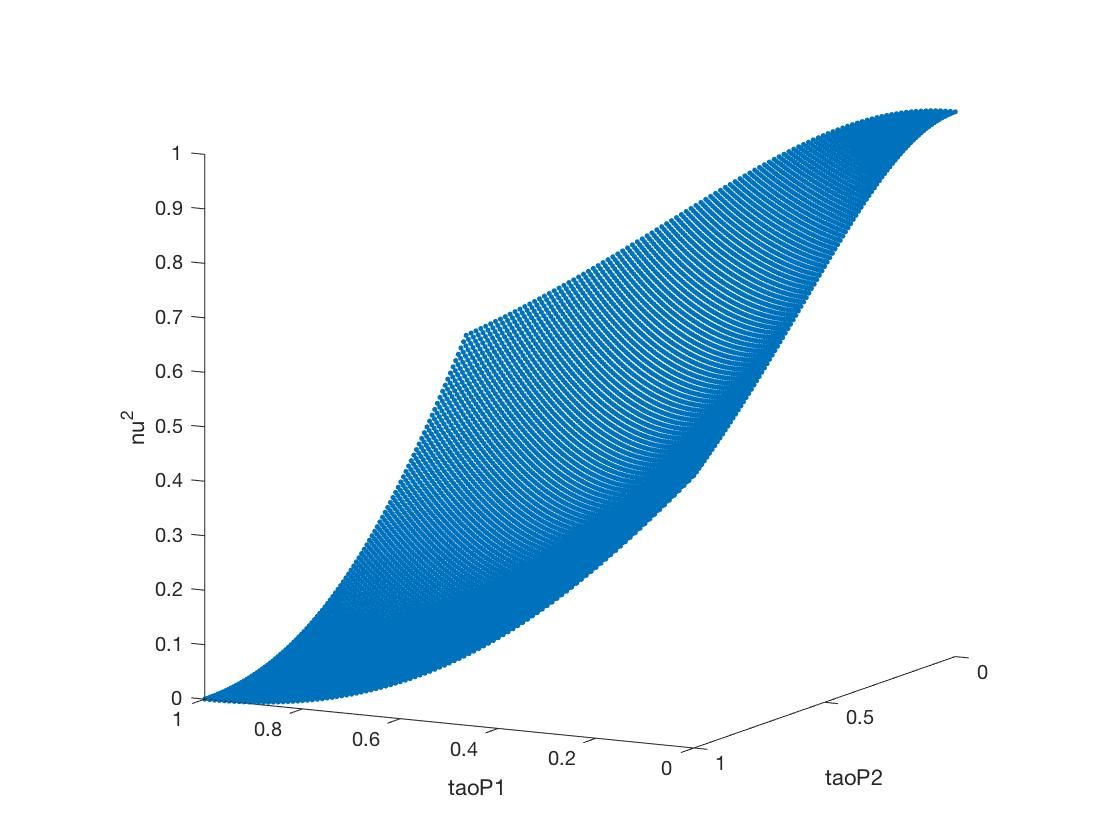
\includegraphics[width=9cm]{images/filter1_1.jpg}
  \caption{График $\nu^2$, построенный по \eqref{filter1_max}.}
  \label{fig:sub2}
\end{subfigure}
\caption{График зависимости $\nu^2$ от $\tau_{p1}, \tau_{p2}$.}
\label{fig:filter1_fig}
\end{figure}

%%%%%%%%%%%%%%%%%%%%%%%%%%%%%%%%%%%%%%%%%%%%%%%%%%%%%%%%%%%%%%%%%%%%%%%
%%%%%%%                      ФИЛЬТР 2                           %%%%%%%
%%%%%%%%%%%%%%%%%%%%%%%%%%%%%%%%%%%%%%%%%%%%%%%%%%%%%%%%%%%%%%%%%%%%%%%

\pagebreak
\subsection{Оценка полосы захвата для систем ФАПЧ с фильтром $\frac{(1+\tau_{z1}s)^2}{(1+\tau_{p1}s)^2}$}
Оценим полосу захвата для систем ФАПЧ с фильтром, определяемым передаточной функцией:
 \begin{equation}\label{filter2}
 \begin{aligned}
W(s) = \frac{(1+\tau_{z1}s)^2}{(1+\tau_{p1}s)^2}, \quad 0<\tau_{p1},\tau_{z1} < 1, \quad \tau_{p1} \neq \tau_{z1}.
 \end{aligned}
\end{equation}
Найдем $\varepsilon, \delta, \varkappa, \tau$ так, чтобы максимизировать $\nu$. Для этого подставим \eqref{filter2} в \eqref{first_th_eq} и перенесем все в левую часть неравенства. Сделаем замену $t = s^2$. В результате преобразований \eqref{first_th_eq} принимает следующий вид:
 \begin{equation}\label{second_condition}
 \begin{aligned}
&\tau_{p1}^4\tau t^3 +(- \tau_{z1}^4\varepsilon - \tau_{z1}^4\tau + 2\tau_{p1}^2\tau- \tau_{p1}^4\delta + \tau_{z1}^2\tau_{p1}^2\varkappa)t^2 +\\
&+( \tau- \tau_{z1}^2\varkappa - 2\tau_{z1}^2\varepsilon - \tau_{p1}^2\varkappa- 2\tau_{z1}^2\tau + 4\tau_{z1}b\varkappa- 2\tau_{p1}^2\delta)t + \\
&+ (\varkappa-\varepsilon - \tau - \delta)  \geqslant 0, \quad \forall t \in \mathbb{R_+}.
 \end{aligned}
\end{equation}
Положим в \eqref{second_condition} $\tau = 0$. Не умаляя общности можем считать $\varkappa = 1$. Тогда \eqref{second_condition} принимает вид:
 \begin{equation}\label{second_condition_tau_zero}
 \begin{aligned}
&(\tau_{z1}^2\tau_{p1}^2\ - \tau_{z1}^4\varepsilon - \tau_{p1}^4\delta)t^2 +( 4\tau_{z1}\tau_{p1} - \tau_{z1}^2 - 2\tau_{z1}^2\varepsilon - \tau_{p1}^2 - 2\tau_{p1}^2\delta)t + \\
&+ (1-\varepsilon - \delta)  \geqslant 0, \quad \forall t \in \mathbb{R_+}.
 \end{aligned}
\end{equation}
Для того чтобы выполнялось \eqref{second_condition_tau_zero} потребуем положительность коэффициентов при $t$, $t^2$ и положительность свободного коэффициента: 
 \begin{equation}\label{filter2_1_area}
 \begin{aligned}
&\tau_{z1}^2\tau_{p1}^2 - \tau_{z1}^4\varepsilon - \tau_{p1}^4\delta \geqslant 0,\\
&4\tau_{z1}\tau_{p1} - \tau_{z1}^2 - 2\tau_{z1}^2\varepsilon - \tau_{p1}^2 - 2\tau_{p1}^2\delta \geqslant 0,\\
&1-\varepsilon - \delta \geqslant 0.
 \end{aligned}
\end{equation}

Оценка $\nu$ будет наибольшей, если параметры $\varepsilon$, $\delta$ лежат на границе допустимой области \eqref{filter2_1_area} и $\delta > 0$, $\varepsilon > 0$. Граница допустимой области является  выпуклым многоугольником, ограниченным прямыми $\delta = 0$, $\varepsilon = 0$ и
 \begin{equation}\label{filter2_1_area_border}
\begin{aligned}
\varepsilon(\delta)=z^2 - z^4\delta \text{,} \quad \varepsilon(\delta)=q - z^2\delta \text{,}
\quad \varepsilon(\delta)=1 - \delta \text{,}
\end{aligned}
\end{equation}
где $z = \frac{\tau_{p1}}{\tau_{z1}}$, $q = 2z - \frac{1}{2} - \frac{1}{2}z^2$. Найдем точки пересечения прямых \eqref{filter2_1_area_border}:
  \begin{equation}
 \begin{aligned}
&\delta = \frac{1}{1+z^2}, \quad \varepsilon = \frac{z^2}{1+z^2};\\
&\delta = \frac{1-q}{1-z^2}, \quad  \varepsilon = \frac{q-z^2}{1-z^2};\\
&\delta = \frac{z^2-q}{z^4-z^2}, \quad  \varepsilon = z^2 - \frac{z^2(z^2-q)}{z^2-1}.\\
 \end{aligned}
\end{equation}
Положим $4\varepsilon\delta$ как максимум по всем граням многоугольника. Тогда $4\varepsilon\delta$ определяется одним из следующих соотношений в зависимости от того, где достигается максимум: на грани или вершинах многоугольника:
 \begin{equation}\label{filter2_max}
\begin{aligned}
\frac{q^2}{z^2}\text{,} \quad 1 \text{,} \quad \frac{4z^2}{1+z^2} \text{,} \quad \frac{4(1-q)(q-z^2)}{1-z^2} \text{,} \quad \frac{z^2-q}{z^2-1} - \left(\frac{z^2-q}{z^2-1}\right)^2.
\end{aligned}
\end{equation}

%  \begin{figure}[H]
%\begin{subfigure}{.5\textwidth}
%  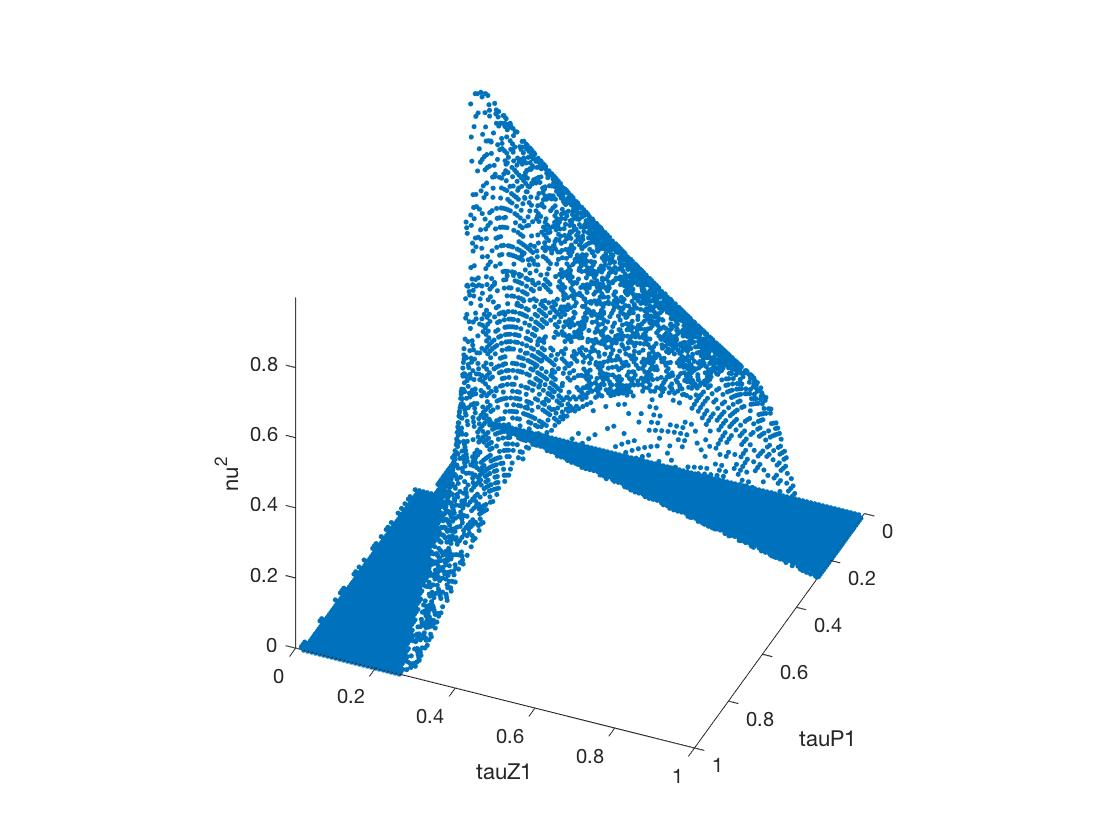
\includegraphics[width=9cm]{images/filter2_tau0_1e.jpg}
%  \caption{Численное приближение в MATLAB}
%  \label{filter2:sub1}
%\end{subfigure}%
% \begin{subfigure}{.5\textwidth}
%  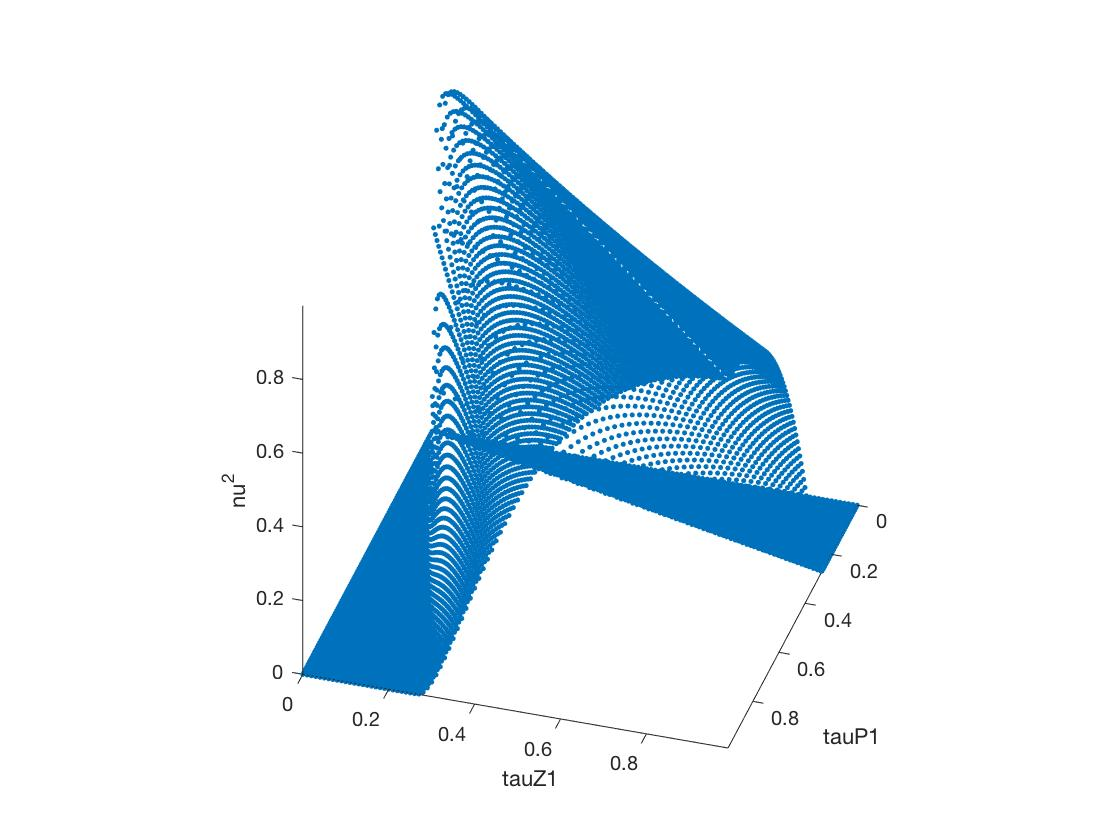
\includegraphics[width=9cm]{images/filter2_tau0_1.jpg}
%  \caption{Вычисленный график}
%  \label{filter2:sub2}
%\end{subfigure}%
%\caption{График зависимости $\nu^2$ от $\tau_{p1}, \tau_{p2}$}
%\label{filter2:filter2_fig}
%\end{figure}


\begin{figure}[H]
\centering
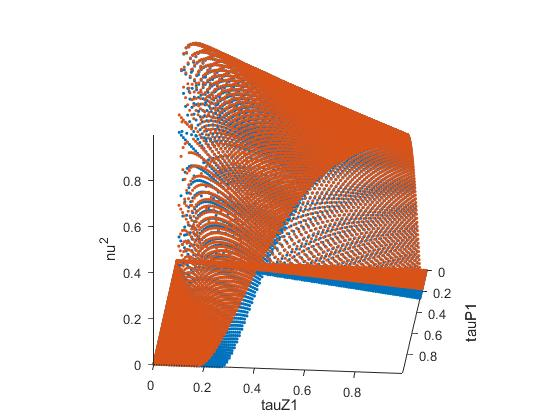
\includegraphics[width=9cm]{images/filter2_agregated.jpg}
\caption{График зависимости $\nu^2$ от $\tau_{p1}, \tau_{p2}$. Красным цветом представлена численная оценка $\nu^2$ согласно \eqref{first_th_eq}, \eqref{second_th_eq} в MATLAB с помощью функции fmincon. Синим цветом представлен график $\nu^2$, построенный по \eqref{filter2_max}, как максимум по всем граням многоугольника.}
\end{figure}

%%%%%%%%%%%%%%%%%%%%%%%%%%%%%%%%%%%%%%%%%%%%%%%%%%%%%%%%%%%%%%%%%%%%%%%
%%%%%%%                      ФИЛЬТР 3                           %%%%%%%
%%%%%%%%%%%%%%%%%%%%%%%%%%%%%%%%%%%%%%%%%%%%%%%%%%%%%%%%%%%%%%%%%%%%%%%

\pagebreak
\subsection{Оценка полосы захвата для систем ФАПЧ с фильтром $\frac{(1+\tau_{z1}x)(1+\tau_{z2}x)}{(1+\tau_{p1}x)(1+\tau_{p2}x)}$}
Оценим полосу захвата для систем ФАПЧ с фильтром, определяемым передаточной функцией:
 \begin{equation}\label{filter3}
 \begin{aligned}
W(s) = \frac{(1+\tau_{z1}s)(1+\tau_{z2}s)}{(1+\tau_{p1}s)(1+\tau_{p2}s)}, \enskip 0<\tau_{pi},\tau_{zj} < 1, \enskip \tau_{pi} \neq \tau_{zj}, \enskip i,j=1,2.
 \end{aligned}
\end{equation}
Введем обозначения:
 \begin{equation}
 \begin{aligned}
\alpha_1 = \tau_{p1} + \tau_{p2}\text{,}\quad 
\alpha_2 = \tau_{p1}\tau_{p2}\text{,}\quad 
\beta_1 = \frac{\tau_{z1}+\tau_{z2}}{\tau_{p1}+\tau_{p2}}\text{,}\quad 
\beta_2 = \frac{\tau_{z1}\tau_{z2}}{\tau_{p1}\tau_{p2}}.
 \end{aligned}
\end{equation}
Тогда \eqref{filter3} принимает вид:
 \begin{equation}\label{filter3-1}
 \begin{aligned}
W(s) = \frac{1+\alpha_1\beta_1s + \alpha_2\beta_2s^2}{1+\alpha_1s + \alpha_2s^2}.
 \end{aligned}
\end{equation}
Положим:
 \begin{equation}\label{restriction-1}
 \begin{aligned}
\beta_1 < \beta_2 < 1.
 \end{aligned}
\end{equation}
Найдем $\varepsilon, \delta, \varkappa, \tau$ так, чтобы максимизировать $\nu$. Для этого подставим \eqref{filter3-1} в \eqref{first_th_eq} и перенесем все в левую часть неравенства. Сделаем замену переменной $t = s^2$. В результате преобразований \eqref{first_th_eq} принимает следующий вид:
 \begin{equation}\label{filter3-th_first-1}
 \begin{aligned}
&\alpha_2^2\tau t^3 + (\alpha_1^2\tau - 2\alpha_2\tau - \alpha_2^2\delta - \alpha_2^2\beta_2^2\varepsilon - \alpha_2^2\beta_2^2\tau + \alpha_2^2\beta_2\varkappa)t^2 +\\
&+ (\tau - \alpha_2\varkappa + 2\alpha_2\delta - \alpha_1^2\delta - \alpha_1^2\beta_1^2\varepsilon - \alpha_1^2\beta_1^2\tau - \alpha_2\beta_2\varkappa + 2\alpha_2\beta_2\varepsilon + \\
&+2\alpha_2\beta_2\tau + \alpha_1^2\beta_1\varkappa)t + \varkappa - \varepsilon - \tau - \delta \geqslant 0, \quad \forall t \in \mathbb{R_+}.
 \end{aligned}
\end{equation}
Положим $\tau = 0$. Не умаляя общности можем считать $\varkappa = 1$. Тогда \eqref{filter3-th_first-1} принимает вид:
 \begin{equation}\label{filter3-th_first-2}
 \begin{aligned}
&(-\varepsilon\alpha_2^2\beta_2^2 + \alpha_2^2\beta_2 - \delta\alpha_2^2)t^2 + (-\varepsilon\alpha_1^2\beta_1^2 + \alpha_1^2\beta_1 - \delta\alpha_1^2 - \alpha_2 + 2\alpha_2\delta - \alpha_2\beta_2 +\\
&+ 2\alpha_2\beta_2\varepsilon)t + 1 - \varepsilon - \delta \geqslant 0, \quad \forall t \in \mathbb{R_+}.
 \end{aligned}
\end{equation}
Заметим, что $\varepsilon \leqslant 1 - \delta$ является необходимым условием справедливости \eqref{filter3-th_first-2}. Для максимизации $\nu$ положим $\varepsilon = 1-\delta$, тогда:
 \begin{equation}\label{filter3-3}
 \begin{aligned}
&(\alpha_2^2\beta_2 - \alpha_2^2\delta - \alpha_2^2\beta_2^2 + \alpha_2^2\beta_2^2\delta)t + \alpha_2\beta_2 - \alpha_2 + 2\alpha_2\delta + \alpha_1^2\beta_1 - \alpha_1^2\delta - \alpha_1^2\beta_1^2 + \\
&\alpha_1^2\beta_1^2\delta - 2\alpha_2\beta_2\delta \geqslant 0, \quad \forall t \in \mathbb{R_+}
 \end{aligned}
\end{equation}
Необходимым и достаточным условием справедливости \eqref{filter3-3} является неотрицательность коэффициента при $t$ и свободного коэффициента:
 \begin{equation}\label{filter3-restriction1}
 \begin{aligned}
&\alpha_2^2\beta_2 - \alpha_2^2\delta - \alpha_2^2\beta_2^2 + \alpha_2^2\beta_2^2\delta \geqslant 0,\\ 
&\alpha_2\beta_2 - \alpha_2 + 2\alpha_2\delta + \alpha_1^2\beta_1 - \alpha_1^2\delta - \alpha_1^2\beta_1^2 + \alpha_1^2\beta_1^2\delta - 2\alpha_2\beta_2\delta \geqslant 0.
 \end{aligned}
\end{equation}
Из \eqref{filter3-restriction1} выразим $\delta$:
 \begin{align}
&\delta \leqslant \frac{\beta_2}{1+\beta_2}, \label{t_coef}\\
&\delta \leqslant \frac{\alpha_1^2(1-\beta_1)\beta_1 - \alpha_2(1-\beta_2)}{\alpha_1^2(1-\beta_1^2) - 2\alpha_2(1-\beta_2)}. \label{free_coef}
 \end{align}
Потребуем положительность числителя \eqref{free_coef}, что равносильно следующему условию:
\begin{equation}\label{filter3-restriction2}
 \begin{aligned}
\alpha_1^2 > \frac{\alpha_2(1-\beta_2)}{\beta_1(1-\beta_1)}.
 \end{aligned}
 \end{equation}
Покажем, что это условие гарантирует положительность знаменателя \eqref{free_coef}:
\begin{equation}
 \begin{aligned}
&\alpha_1^2(1-\beta_1^2) - 2\alpha_2(1-\beta_2) > \frac{\alpha_2(1-\beta_2)}{\beta_1}(1+\beta_1) - 2\alpha_2(1-\beta_2) =\\
&= \frac{\alpha_2(1-\beta_2)(1 - \beta_1)}{\beta_1} > 0.
 \end{aligned}
\end{equation}
Покажем, что условие \eqref{free_coef} и \eqref{filter3-restriction2} влечет выполнение \eqref{t_coef}. Из условия \eqref{filter3-restriction2} следует, что функция \eqref{free_coef}, как функция от  $\beta_1$ строго возрастает, на допустимой области параметров, тогда:
 \begin{align}
\frac{\alpha_1^2(1-\beta_1)\beta_1 - \alpha_2(1-\beta_2)}{\alpha_1^2(1-\beta_1^2) - 2\alpha_2(1-\beta_2)} < \frac{\alpha_1^2\beta_2 - \alpha_2}{\alpha_1^2(1+\beta_2) - 2\alpha_2} < \frac{\beta_2}{1+\beta_2}.
 \end{align}
Так как максимальное значение $\nu$ достигается на границе допустимой области, положим:
 \begin{equation}\label{filter3_positive_numerator}
 \begin{aligned}
\delta = \frac{\alpha_1^2(1-\beta_1)\beta_1 - \alpha_2(1-\beta_2)}{\alpha_1^2(1-\beta_1^2) - 2\alpha_2(1-\beta_2)}.
 \end{aligned}
 \end{equation}
В результате вычислений получили, что максимальное значение $\nu$ будет при следующем наборе параметров:
\begin{equation}\label{filter3-params}
 \begin{aligned}
 \tau = 0 \text{,} \quad
 \varkappa = 1 \text{,} \quad
 \varepsilon = 1-\delta \text{,} \quad
 \delta = \frac{\alpha_1^2(1-\beta_1)\beta_1 - \alpha_2(1-\beta_2)}{\alpha_1^2(1-\beta_1^2) - 2\alpha_2(1-\beta_2)}.
 \end{aligned}
\end{equation}
Тогда, подставив \eqref{filter3-params} в \eqref{first_th_eq} и применив \eqref{second_th_eq}, получим оценку:
 \begin{equation}
 \begin{aligned}
\nu^2 < 4\frac{[\alpha_1^2(1-\beta_1) - \alpha_2(1-\beta_2)][\alpha_1^2(1-\beta_1)\beta_1 - \alpha_2(1-\beta_2)]}{[\alpha_1^2(1-\beta_1^2) - 2\alpha_2(1-\beta_2)]^2}.
 \end{aligned}
 \end{equation}
 
\pagebreak
\section{Заключение}
В рамках данной работы были рассмотрены следующие передаточные функции фильтров: 
 \begin{align}
&W(s) = \frac{1}{(1+\tau_{p1}s)(1+\tau_{p2}s)},\label{first}\\[5pt]
&W(s) = \frac{(1+\tau_{z1}s)^2}{(1+\tau_{p1}s)^2},\label{second}\\[5pt]
&W(s) = \frac{(1+\tau_{z1}x)(1+\tau_{z2}x)}{(1+\tau_{p1}x)(1+\tau_{p2}x)},\label{third}\\
&0<\tau_{pi},\tau_{zj} < 1, \quad \tau_{pi} \neq \tau_{zj}, \quad i=1,2, \quad j=1,2.
 \end{align}
 Для \eqref{first}, \eqref{second} были получены аналитические оценки полосы захвата, которые были подтверждены численно. Полоса захвата систем ФАПЧ с фильтром, определяемым передаточной функцией \eqref{third} исследовалась ранее Леоновым~Г.\:А. \cite{kuznetsov}. Для нее был восстановлен вывод. 
 
 В настоящее время системы фазовой автоподстройки частоты используются в различных устройствах. Аналитические оценки, полученные в данной работе, могут быть интересны инженерам при проектировании и реализации систем ФАПЧ 3 порядка.
 
 \pagebreak
\specialsection{Листинги}

\lstinputlisting{code/filter1_exact.m}
\lstinputlisting{code/filter1_analytic.m}

\lstinputlisting{code/filter2_exact.m}
\lstinputlisting{code/filter2_analytic.m}
\lstinputlisting{code/maximize.m}
 
\pagebreak
\begin{thebibliography}{20}
\bibitem{ghulam} Ghulam~H.\:R. A mathematical model and simulation of frequency hopping interferences to FM systems // Mathematical and Computer Modelling. 1988. Vol.~11, No~10. P.~988--993.

\bibitem{Microprocessors}
Young~I.\:A., Greason~J.\:K., Wong~K.\:L. A PLL clock generator with 5 to 110 MHz of lock range for microprocessors //  IEEE Journal of Solid-State Circuits. 1992. Vol.~ 27, No.~11. P.~1599-1607

\bibitem{appleton} 
Appleton~E.\:V. The Automatic Synchronization of Triode Oscillators // Proc. Camb. Phil. Soc. 1923. Vol.~21, P.~231--248.

\bibitem{blagov} 
Blagov~M.\:V., Kuznetsova~O.\:A., Kudryashova~E.\:V., Kuznetsov~N.\:V., Mokaev~T.\:N., Mokaev~R.\:N., Yuldashev~M.\:V., Yuldashev~R.\:V. Hold-in, Pull-in and Lock-in Ranges for Phase-locked Loop with Tangential Characteristic of the Phase Detector // Procedia Computer Science. 2019. Vol.~150, P.~558--566.

\bibitem{seledji}
Леонов~Г.\:А., Селеджи~С.\:М. Системы фазовой синхронизации в аналоговой и цифровой схемотехнике. СПб.: <<Невский Диалект>>, 2002. 112~с.

\bibitem{best}  
Best~R.\:E. Phase-Locked Loops: Design, Simulation, and Applications. New York: McGraw-Hill Education, 2007. 421~p.

\bibitem{ashari}
Ashari~Z., Nordin~A.\:N Theoretical Modeling and Simulation of Phase-Locked Loop (PLL) for Clock Data Recovery (CDR) // IIUM Engineering Journal. 2011. Vol.~12, No.~5. P.~105--113.

\bibitem{rao}  
Rao~R.\:B., Kunysz~W., Fante~R., McDonald~K. GPS/GNSS Antennas. Boston: Artech House, 2013. 420~p.

\bibitem{kuznetsov_nonlinear}
Kuznetsov~N.\:V., Leonov~G.\:A., Neittaanmäki~P., Seledzhi~S.\:M., Yuldashev~M.\:V., Yuldashev~R.\:V. Nonlinear Analysis of Phase-Locked Loop // IFAC Proceedings Volumes. 2010. Vol.~43, No.~11. P.~34--38.

\bibitem{thirdOrderPLL} 
Feng~L., Wu~C., Jin~B., Wu~Z. A Passive Third-order Cascade PLL Filter // Trans Tech Publications. 2011. Vol. 255--260. P.~2262--2266.

\bibitem{UsageOfThirdOrder1}
Ujwala~A. Belorkar, Ladhake~S.\:A. Design of Low Power Phase Locked Loop (PLL) Using 45NM VLSI Technology // International journal of VLSI design \& Communication Systems  (LSICS). 2010. Vol.~1, No.~2. P.~1-11.

\bibitem{shahgildyan}  
Шахгильдян~В.\:В., Ляховкин~А.\:А. Системы фазовой автоподстройки частоты. М.:~Изд-во <<Связь>>, 1972. 447~с.

\bibitem{kuznetsov_article} 
Kuznetsov~N.\:V., Leonov~G.\:A., Yuldashev~M.\:V., Yuldashev~R.\:V. Hold-In, Pull-In, and Lock-In Ranges of PLL Circuits: Rigorous Mathematical Definitions and Limitations of Classical Theory // Transactions on Circuits and Systems I: Regular Papers. 2015. Vol.~62, No~10. P.~2454--2464.
 
\bibitem{kuznetsov}  
Leonov~G.\:A., Kuznetsov~N.\:V. Nonlinear mathematical models of phase-locked loops : stability and oscillations. Cambridge: Cambridge Scientific Publishers, 2014. 218~p.

\bibitem{kaplan} 
Kaplan~D.\:E., Hegarty~J.\:C. Understanding GPS: Principles And Applications. Boston: Artech House, 2006. 724~p.

\bibitem{leonov}  
Leonov~G.\:A., Reitmann~V., Smirnova~V.\:B. Non-Local Methods for Pendulum-Like Feedback Systems. Wiesbaden: Vieweg+Teubner Verlag, 1992. 242~p.

\end{thebibliography}
\end{document}  
% КОНЕЦ ДОКУМЕНТА !